\documentclass[a4paper,12pt]{article}

% Pacchetti fondamentali
\usepackage[utf8]{inputenc}   % Codifica caratteri
\usepackage{babel}
\babelprovide[import, main]{italian}    % Lingua italiana
\usepackage{amsmath}           % Formule matematiche avanzate
\usepackage{graphicx}          % Inserimento immagini
\usepackage{geometry}          % Gestione margini
\geometry{margin=2.5cm}
\usepackage{booktabs}          % Tabelle professionali
\usepackage{physics}
\usepackage{float}
\usepackage{caption}
\usepackage{textcomp}
\usepackage{amssymb}
\usepackage{parskip}
\usepackage{float}

\title{Misura del calore specifico a bassa temperatura}
\author{Eddi Bressan, Davide Conforte}
\date{\today}

\begin{document}

\maketitle
\tableofcontents
\newpage


\section{Obiettivo dell'esperienza}

L'obiettivo dell'esperienza è la determinazione sperimentale del calore latente di evaporazione
dell'azoto liquido e la successiva misura del calore specifico medio a pressione costante di due
campioni solidi: grafite e piombo.


\section{Cenni teorici}
\subsection{Calore latente di vaporizzazione dell'azoto}

L'azoto liquido assorbe calore $\Delta Q_0$ dall'ambiente e quindi evapora con una velocità
$\frac{\Delta m }{\Delta t}$ che, se le condizioni di contatto termico con l'ambiente rimangono invariate,
si può dire costante:
\begin{equation*}
    W_0 = \frac{\Delta Q_0}{\Delta t} = \frac{\lambda_f \Delta m}{\Delta t}
\end{equation*}
dove $\lambda_f$ è il calore latente di vaporizzazione dell'azoto.
Da cui:
\begin{equation*}
    \Delta m = \frac{W_0}{\lambda_f} \Delta t
\end{equation*}
Quando si fa passare corrente nel circuito con la resistenza a contatto con l'azoto liquido, la
quantità di calore assorbita aumenta di una frazione corrispondente alla potenza dissipata dalla
resistenza $W_R$:
\begin{equation*}
    W_0 + W_R = \frac{\Delta Q_0 + \Delta Q_R}{\Delta t}
\end{equation*}
Da cui:
\begin{equation*}
    \Delta m = \frac{W_0 + W_R}{\lambda_f} \Delta t
\end{equation*}
Le pendenze delle rette con il circuito aperto (senza corrente SC) e con il circuito chiuso
(con corrente CC) corrispondono alla variazione di massa nell'unità di tempo:
\begin{align*}
    \left. \frac{\Delta m}{\Delta t} \right|_{SC} &= \frac{W_0}{\lambda_f} \\
    \left. \frac{\Delta m}{\Delta t} \right|_{CC} &= \frac{W_0}{\lambda_f} + \frac{W_R}{\lambda_f}
\end{align*}

Sottraendo alla pendenza misurata con la corrente quella misurata senza, posso isolare il solo
contributo della resistenza:
\begin{equation*}
    \left. \frac{\Delta m}{\Delta t} \right|_{CC} - \left. \frac{\Delta m}{\Delta t} \right|_{SC} = \frac{W_R}{\lambda_f} = \frac{V I}{\lambda_f}
\end{equation*}
dove V e I sono rispettivamente la differenza di tensione e l'intensità di corrente misurate con
l'amperometro e il voltmetro (in serie e in parallelo con la resistenza).

In questo modo si riesce a ottenere una misura del calore latente di vaporizzazione dell'azoto:
\begin{equation*}
    \lambda_f = \frac{V I}{\left. \frac{\Delta m}{\Delta t} \right|_{CC} - \left. \frac{\Delta m}{\Delta t} \right|_{SC}}
\end{equation*}
con errore:
\begin{align*}
    \Delta \lambda_f &= \Delta V \left| \frac{I}{\left. \frac{\Delta m}{\Delta t} \right|_{CC} - \left. \frac{\Delta m}{\Delta t} \right|_{SC}} \right| + \Delta I \left| \frac{V}{\left. \frac{\Delta m}{\Delta t} \right|_{CC} - \left. \frac{\Delta m}{\Delta t} \right|_{SC}} \right| + \\
    &\quad + \left[ \Delta\left(\left. \frac{\Delta m}{\Delta t} \right|_{CC}\right) + \Delta \left( \left. \frac{\Delta m}{\Delta t} \right|_{SC} \right) \right] \left| \frac{VI}{\left( \left. \frac{\Delta m}{\Delta t} \right|_{CC} - \left. \frac{\Delta m}{\Delta t} \right|_{SC} \right)^2} \right|
\end{align*}

In alternativa possiamo usare il metodo grafico.
Indicando con $t_{start}$ e $t_{stop}$ gli istanti di accensione e di spegnimento, si tracciano le
rette per la fase 1 (prima dell'accensione) e per la fase 3 (dopo l'accensione) e le si estrapola
a $t_m = \frac{t_{start} + t_{stop}}{2}$.

Poi si tracciano le rette a pendenza massima e minima, estrapolandole allo stesso $t_m$ e
si misurano i valori di $\Delta \left( \left.\Delta m \right|_{fase 1} \right)$ e $\Delta \left( \left.\Delta m \right|_{fase 3} \right)$.

Si misurano quindi la distanza tra le due rette al tempo $t_m$ di valore $\Delta m$ e l'errore $\Delta \left( \Delta m \right) = \Delta \left( \left.\Delta m \right|_{fase 1} \right) + \Delta \left( \left.\Delta m \right|_{fase 3} \right)$.

Si può così misurare il calore latente di vaporizzazione:
\begin{equation*}
    \lambda_f = \frac{V I}{\Delta m} (t_{stop} - t_{start}) = \frac{V I \Delta t}{\Delta m}
\end{equation*}
con errore:
\begin{equation*}
    \Delta \lambda_f = \lambda_f \left( \frac{\Delta V}{V} + \frac{\Delta I}{I} + \frac{\Delta (\Delta m)}{(\Delta m)} + \frac{\Delta (\Delta t)}{(\Delta t)} \right)
\end{equation*}
Per questo metodo, si possono ricavare le equazioni delle rette con il metodo dei minimi quadrati
lineari per trovare il migliore fit lineare.


\subsection{Calore specifico medio}

Il calore trasferito da n moli di un materiale all'azoto liquido ad una certa temperatura è:
\begin{equation*}
    dQ = nc(T)dT
\end{equation*}
con c calore specifico del materiale alla temperatura T.

Nell'intervallo tra la temperatura ambiente $T_a$ e la temperatura di vaporizzazione dell'azoto
liquido $T_f$ si ha:
\begin{equation*}
    Q = n \int_{T_a}^{T_f} c(T)dT \approx n \sum \frac{c(T_k) + c(T_{k+1})}{2} \abs{T_{k+1} - T_k}
\end{equation*}
Si definisce il calore specifico medio nell'intervallo di temperatura come:
\begin{equation*}
    \bar{c_x} = \frac{1}{n} \frac{Q}{\abs{T_a - T_f}} = \frac{1}{\abs{T_a - T_f}} \sum \frac{c(T_k) + c(T_{k+1})}{2} \abs{T_{k+1} - T_k}
\end{equation*}
Formula che può essere utilizzata per il calcolo approssimato degli integrali (regola del trapezio)
per calcolare la capacità termica molare media per le sostanze di nostro interesse.

Pertanto, usando il metodo grafico e estrapolando le rette per la fase 1 (prima dell'immersione
della sostanza) e per la fase 3 (dopo la stabilizzazione della perdita di massa nel tempo) come
descritto sopra, si può calcolare il calore specifico medio (J/(Kg K)) come:
\begin{equation*}
        \bar{c_x} = \frac{\Delta m \lambda_f}{m_x (T_f - T_a)}
\end{equation*}
con $m_x$ la massa della sostanza. L'errore di $c_x$ è dato da:
\begin{equation*}
    \Delta c_x = \left( \frac{\Delta (\Delta m)}{(\Delta m)} + \frac{\Delta \lambda_f}{\lambda_f} + \frac{\Delta m_x}{m_x} + \frac{2 \Delta T}{(T_a - T_f)} \right) c_x
\end{equation*}
Di seguito si riporta una tabella di calori specifici molari a diverse temperature, su cui possiamo basarci per 
fare predizioni utili allo svolgimento della esperienza:
\begin{table}[H]
\centering
\begin{tabular}{ccc}
\toprule
\textbf{T} (K) & \textbf{C} ($\text{cal}\cdot\text{mol}^{-1}\cdot\text{K}^{-1}$) & \textbf{Pb} ($\text{cal}\cdot\text{mol}^{-1}\cdot\text{K}^{-1}$) \\
\midrule
70  & 0.221 & 5.54 \\
80  & 0.278 & 5.64 \\
90  & 0.339 & 5.74 \\
100 & 0.402 & 5.84 \\
120 & 0.539 & 5.94 \\
140 & 0.689 & 5.99 \\
160 & 0.849 & 6.09 \\
180 & 1.019 & 6.14 \\
200 & 1.188 & 6.19 \\
220 & 1.36  & 6.24 \\
240 & 1.54  & 6.29 \\
260 & 1.71  & 6.34 \\
280 & 1.88  & 6.38 \\
300 & 2.05  & 6.44 \\
\bottomrule
\end{tabular}
\end{table}



\iffalse
\section{Apparato sperimentale}

Per la misura del calore latente di vaporizzazione è stato realizzato un circuito composto da:
\begin{itemize}
    \item Resistenza elettrica da $10.3 \pm 0.1 \Omega$
    \item Generatore di corrente continua
    \item Voltmetro con errore di sensibilità ....DA INSERIRE....
    \item Amperometro con errore di sensibilità ....DA INSERIRE....
\end{itemize}

Sono stati utilizzati anche i seguenti strumenti e materiali:
\begin{itemize}
    \item Vaso Dewar
    \item Azoto liquido ($LN_2$)
    \item Campione di piombo ($Pb$)
    \item Campione di grafite ($C$)
    \item Termometro a termocoppia con errore di sensibilità ....DA INSERIRE....
    \item Bilancia elettronica con errore di sensibilità ....DA INSERIRE....
    \item Cronometro digitale con errore di sensibilità ....DA INSERIRE....
\end{itemize}




\section{Procedura sperimentale}

Come procedimento preliminare all'esperienza, è stata calcolata la potenza dissipata dal circuito necessaria
a indurre l'evaporazione di una massa di circa 10g di azoto liquido in un intervalllo di 5 minuti.
Il generatore di corrente è stato conseguentemente impostato sui valori di tensione e intensità di
corrente atti a garantire tale potenza.

Successivamente, misurata la temperatura ambiente, si è proceduto alla determinazione del calore 
specifico medio dei campioni di piombo e grafite, utilizzando i dati riportati nella tabella in
precedenza.

Infine, attraverso un bilancio termido basato sulla temperatura di equilibrio raggiunta, è stata
stimata la quantità di azoto evaporato in seguito al contatto con i materiali analizzati.

\subsection{Calore latente di vaporizzazione dell'azoto}
Si inserisce l'azoto liquido nel vaso Dewar insieme alla resistenza elettrica e si posiziona il tutto
sopra la bilancia elettronica.

Si misura così la massa del sistema ogni 20 secondi per 5 minuti. Terminati i 5 minuti si accende il circuito
e si continua a misurare la massa ogni 10 secondi per 5 minuti. Infine si spegne il circuito e si continua
a misurare la massa ogni 20 secondi per 5 minuti.


\subsection{Calore specifico medio}

Il seguente procedimento va eseguito per il campione di piombo e quello di grafite.

Si misura la massa del campione, poi si posiziona il vaso Dewar con l'azoto liquido sulla bilancia
elettronica insieme al campione che però resta posizionato al di fuori del vaso Dewar, sopra il piatto della bilancia.

Si misura così la massa del sistema ogni 20 secondi per 5 minuti. Si introduce poi il campione nell'azoto
liquido e si continua a misurare la massa del sistema ogni 10 secondi finché il campione e l'azoto liquido
non raggiungono l'equilibrio termico tra loro e si registra una perdita di massa dovuta solamente allo scambio
termico con l'ambiente.

\section{Presa dati}
In seguito sono riportate tutte le misure raccolte durante l'esperienza.

Per avere una perdita pari a 10g di azoto in 5 minuti, è stato calcolata una potenza necessaria di:
\begin{equation*}
    W = VI = 6.67W
\end{equation*}
Pertanto è stato misurato:

\begin{table}[h]
    \centering
    \begin{tabular}{|c|c|} \hline
        V (V) & 8.29 \\ \hline
        I (A) & 0.80 \\ \hline
    \end{tabular}
\end{table}

Le masse misurate dei campioni sono:

\begin{table}[h]
    \centering
    \begin{tabular}{|c|c|} \hline
        Piombo (g) & 38.48 \\ \hline
        Grafite (g) & 17.17 \\ \hline
    \end{tabular}
\end{table}

Ricaviamo così il numero di moli:
\begin{table}[h]
    \centering
    \begin{tabular}{|c|c|c|c|} 
        \hline
        \multicolumn{2}{|c|}{\textbf{Piombo}} & \multicolumn{2}{c|}{\textbf{Grafite}} \\ \hline
        M (g/mol) & 207.2 & M (g/mol) & 12.01 \\ \hline
        n (mol) & 1.430 & n (mol) & 0.186 \\ \hline
    \end{tabular}
\end{table}

Avendo misurato $T_a = 294.6K$, sapendo che $T_f = 77.4K$ e avendo supposto lineare la variazione di calore
specifico negli intervalli indicati nella tabella, abbiamo calcolato il calore specifico medio e la perdita
di massa: 


DAVIDE AIUTO!!!!!!!!!!!!!!
\begin{table}[H]
    \centering
    % Prima tabella
    \begin{minipage}{0.45\textwidth}
        \centering
        \begin{tabular}{|c|c|}
            \hline
            \multicolumn{2}{|c|}{\textbf{Piombo}} \\ \hline
            $C_x$ (cal/(mol K)) & Dato 2 \\ 
            $C_x$ (J/(Kg K)) & Dato 4 \\ \hline
            $\Delta m$ (g) & Dato 6 \\ \hline
        \end{tabular}
        \caption{Prima tabella}
    \end{minipage}
    \hfill
    % Seconda tabella
    \begin{minipage}{0.45\textwidth}
        \centering
        \begin{tabular}{|c|c|}
            \hline
            \multicolumn{2}{|c|}{\textbf{Grafite}} \\ \hline
            $C_x$ (cal/(mol K)) & Dato 2 \\ 
            $C_x$ (J/(Kg K)) & Dato 4 \\ \hline
            $\Delta m$ (g) & Dato 6 \\ \hline
        \end{tabular}
        \caption{Seconda tabella}
    \end{minipage}
\end{table}
DAVIDE AIUTO!!!!!!!!!!!!!
Abbiamo quindi una perdita di massa totale XYZ, escludendo quella continuamente persa a causa dello scambio
termico con l'ambiente.


\subsection{Calore latente di vaporizzazione dell'azoto}

\begin{table}[H]
    \centering
    % Prima tabella
    \begin{minipage}[t]{0.30\textwidth}
        \vspace{0pt}
        \centering
        \begin{tabular}{|c|c|}
            \hline
            \multicolumn{2}{|c|}{\textbf{Senza corrente}} \\ \hline
            t (s) & m (g) \\ \hline
            0.00 & 1606.58 \\ \hline
            20.35 & 1606.20 \\ \hline
            40.41 & 1605.65 \\ \hline
            60.11 & 1605.25 \\ \hline
            80.62 & 1604.75 \\ \hline
            100.93 & 1604.30 \\ \hline
            122.01 & 1603.87 \\ \hline
            142.22 & 1603.38 \\ \hline
            162.67 & 1602.96 \\ \hline
            184.60 & 1602.41 \\ \hline
            204.96 & 1602.00 \\ \hline
            225.69 & 1601.55 \\ \hline
            245.66 & 1601.06 \\ \hline
            265.77 & 1600.65 \\ \hline
            289.19 & 1600.16 \\ \hline
            306.70 & 1599.70 \\ \hline
        \end{tabular}
    \end{minipage}
    \hfill
    % Seconda tabella
    \begin{minipage}[t]{0.30\textwidth}
        \vspace{0pt}
        \centering
        \begin{tabular}{|c|c|}
            \hline
            \multicolumn{2}{|c|}{\textbf{Con corrente}} \\ \hline
            t (s) & m (g) \\ \hline
            365.48 & 1598.70 \\ \hline
            375.86 & 1598.30 \\ \hline
            386.20 & 1597.50 \\ \hline
            396.84 & 1597.00 \\ \hline
            406.82 & 1596.50 \\ \hline
            417.29 & 1596.00 \\ \hline
            427.53 & 1595.40 \\ \hline
            437.65 & 1594.25 \\ \hline
            456.31 & 1593.77 \\ \hline
            466.67 & 1593.12 \\ \hline
            477.13 & 1592.70 \\ \hline
            487.43 & 1592.09 \\ \hline
            497.75 & 1591.50 \\ \hline
            507.99 & 1590.99 \\ \hline
            518.56 & 1590.40 \\ \hline
            528.98 & 1589.78 \\ \hline
            539.90 & 1589.30 \\ \hline
            550.28 & 1588.80 \\ \hline
            560.86 & 1588.27 \\ \hline
            571.96 & 1587.62 \\ \hline
            582.27 & 1587.08 \\ \hline
            592.65 & 1586.59 \\ \hline
            603.03 & 1585.98 \\ \hline
        \end{tabular}
    \end{minipage}
    \hfill
    % Terza tabella
    \begin{minipage}[t]{0.30\textwidth}
        \vspace{0pt}
        \centering
        \begin{tabular}{|c|c|}
            \hline
            \multicolumn{2}{|c|}{\textbf{Senza corrente}} \\ \hline
            t (s) & m (g) \\ \hline
            623.40 & 1585.16 \\ \hline
            643.85 & 1584.90 \\ \hline
            664.21 & 1584.70 \\ \hline
            684.70 & 1584.40 \\ \hline
            705.06 & 1584.94 \\ \hline
            725.79 & 1584.45 \\ \hline
            746.03 & 1584.02 \\ \hline
            766.48 & 1583.63 \\ \hline
            787.24 & 1583.25 \\ \hline
            807.74 & 1582.80 \\ \hline
            828.15 & 1582.40 \\ \hline
            848.36 & 1582.96 \\ \hline
            868.78 & 1581.55 \\ \hline
            889.21 & 1581.13 \\ \hline
        \end{tabular}
    \end{minipage}
\end{table}
\fi
\section{Determinazione del Calore Latente di Evaporazione dell'Azoto Liquido}

\subsection{Stima Preliminare della Potenza Termica e Dimensionamento Elettrico}
L'esperimento si propone di misurare il calore latente di evaporazione dell'azoto liquido ($\lambda_f$). In via preliminare, è stata effettuata una stima della potenza termica $P$ necessaria a far evaporare una massa di azoto $m = 10\text{ g}$ in un intervallo di tempo $\Delta t = 300\text{ s}$ (pari a 5 minuti). 

Assumendo come valore di riferimento da manuale per il calore latente di evaporazione dell'azoto il valore $L_e \approx 199\text{ J/g}$, la potenza teorica necessaria risulta:
\begin{equation}
P = \frac{Q}{\Delta t} = \frac{m \cdot L_e}{\Delta t} = \frac{10\text{ g} \cdot 199\text{ J/g}}{300\text{ s}} \approx 6.63\text{ W}
\end{equation}

Per fornire tale potenza termica mediante effetto Joule, si è utilizzata una resistenza elettrica nota pari a $R = 10.3\ \Omega$ immersa nel vaso Dewar contenente il liquido. I parametri elettrici di funzionamento (corrente $I$ e tensione $V$) necessari per erogare la potenza target sono stati calcolati invertendo le relazioni della potenza elettrica:
\begin{equation}
I = \sqrt{\frac{P}{R}} = \sqrt{\frac{6.63\text{ W}}{10.3\ \Omega}} \approx 0.802\text{ A}
\end{equation}
\begin{equation}
V = R \cdot I = 10.3\ \Omega \cdot 0.81\text{ A} \approx 8.34\text{ V}
\end{equation}
I valori sperimentali effettivamente impostati sul generatore sono stati fissati a $I \approx 0.81\text{ A}$ e $V \approx 8.3\text{ V}$, corrispondenti a una potenza reale dissipata $W_R = V \cdot I \approx 6.72\text{ W}$.

\subsection{Procedura di Misura a Tre Fasi}
Per isolare la frazione di azoto evaporata a causa della potenza elettrica rispetto a quella dovuta all'interazione termica spontanea con l'ambiente circostante ($W_0$), la presa dati è stata suddivisa in tre fasi temporali consecutive di 5 minuti ciascuna:
\begin{enumerate}
    \item \textbf{Fase I (Circuito Aperto - SC):} Misura della perdita di massa a intervalli di $10 \div 30$ secondi con il circuito spento. Consente di determinare il background termico iniziale dovuto all'ambiente.
    \item \textbf{Fase II (Circuito Chiuso - CC):} Accensione del circuito per 5 minuti e monitoraggio della perdita di massa combinata (ambiente + resistenza) a intervalli più fitti ($10 \div 20$ secondi).
    \item \textbf{Fase III (Circuito Aperto - SC):} Spegnimento del circuito e nuova misura della perdita di massa per altri 5 minuti per valutare eventuali variazioni del background termico spontaneo nel tempo.
\end{enumerate}

\subsection{Analisi Dati: Il Metodo Grafico}
Per l'estrazione del calore latente si è adottato il metodo grafico (o delle estrapolazioni). Definiti $t_{\text{start}}$ e $t_{\text{stop}}$ come gli istanti di accensione e spegnimento della resistenza (estremi della Fase II), si individua l'istante temporale medio:
\begin{equation}
t_m = \frac{t_{\text{start}} + t_{\text{stop}}}{2}
\end{equation}

Si esegue l'estrapolazione lineare delle rette di tendenza della Fase I e della Fase III fino al tempo centrale $t_m$. La distanza verticale tra le due rette valutata in $t_m$ fornisce direttamente la massa netta $\Delta m$ evaporata a causa della sola resistenza elettrica durante l'intera Fase II:
\begin{equation}
\Delta m = m_{\text{Fase I}}(t_m) - m_{\text{Fase III}}(t_m)
\end{equation}

Il calore latente di evaporazione viene quindi calcolato come:
\begin{equation}
\lambda_f = \frac{W_R \cdot \Delta t}{\Delta m} = \frac{V I \Delta t}{\Delta m}
\end{equation}
dove $\Delta t = t_{\text{stop}} - t_{\text{start}}$.

L'incertezza sulla massa netta $\Delta(\Delta m)$ viene stimata tracciando le rette a pendenza massima e minima per le Fasi I e III, estrapolandone i valori a $t_m$:
\begin{equation}
\Delta(\Delta m) = \Delta(\Delta m|_{\text{Fase I}}) + \Delta(\Delta m|_{\text{Fase III}})
\end{equation}

Infine, propagando gli errori per la grandezza $\lambda_f$ espressa come prodotto e quoziente di variabili, l'incertezza assoluta $\Delta \lambda_f$ risulta:
\begin{equation}
\Delta \lambda_f = \lambda_f \left( \frac{\Delta V}{V} + \frac{\Delta I}{I} + \frac{\Delta(\Delta m)}{\Delta m} + \frac{\Delta(\Delta t)}{\Delta t} \right)
\end{equation}

\begin{table}[htbp]
\centering
\caption{Dati sperimentali della variazione di massa dell'azoto liquido, suddivisi analiticamente nelle tre fasi sequenziali dell'esperimento.}
\label{tab:dati_fasi_confronto}
\vspace{0.3cm}
\footnotesize % Ottimizza lo spazio per l'allineamento orizzontale

% --- MINIPAGE FASE I ---
\begin{minipage}[t]{0.31\textwidth}
\centering
\textbf{Fase I: Background Iniziale} \\
\textit{(Circuito Aperto)} \\
\vspace{0.2cm}
\begin{tabular}{cc}
\toprule
\textbf{T (s)} & \textbf{Massa (g)} \\
\midrule
0.00 & 1606.58 \\
20.35 & 1606.20 \\
40.41 & 1605.65 \\
60.11 & 1605.25 \\
80.62 & 1604.75 \\
100.93 & 1604.30 \\
122.01 & 1603.87 \\
142.22 & 1603.38 \\
162.67 & 1602.96 \\
184.60 & 1602.41 \\
204.96 & 1602.00 \\
225.69 & 1601.55 \\
245.66 & 1601.06 \\
265.77 & 1600.65 \\
286.19 & 1600.16 \\
\bottomrule
\end{tabular}
\end{minipage}
\hfill
% --- MINIPAGE FASE II ---
\begin{minipage}[t]{0.33\textwidth}
\centering
\textbf{Fase II: Dissipazione} \\
\textit{(Resistenza Accesa)} \\
\vspace{0.2cm}
\begin{tabular}{cc}
\toprule
\textbf{T (s)} & \textbf{Massa (g)} \\
\midrule
\textbf{306.70} & \textbf{1599.70} \\
365.48 & 1598.70 \\
375.86 & 1598.30 \\
386.20 & 1597.50 \\
396.84 & 1597.00 \\
406.82 & 1596.50 \\
417.29 & 1596.00 \\
427.53 & 1595.40 \\
437.65 & 1594.25 \\
456.31 & 1593.77 \\
466.67 & 1593.12 \\
477.13 & 1592.70 \\
487.43 & 1592.09 \\
497.75 & 1591.50 \\
507.99 & 1590.99 \\
518.56 & 1590.40 \\
528.98 & 1589.78 \\
539.90 & 1589.30 \\
550.28 & 1588.80 \\
560.86 & 1588.27 \\
571.96 & 1587.62 \\
582.27 & 1587.08 \\
592.65 & 1586.59 \\
\textbf{603.03} & \textbf{1585.98} \\
\bottomrule
\end{tabular}
\end{minipage}
\hfill
% --- MINIPAGE FASE III ---
\begin{minipage}[t]{0.31\textwidth}
\centering
\textbf{Fase III: Background Finale} \\
\textit{(Circuito Aperto)} \\
\vspace{0.2cm}
\begin{tabular}{cc}
\toprule
\textbf{T (s)} & \textbf{Massa (g)} \\
\midrule
623.40 & 1585.16 \\
643.85 & 1584.90 \\
664.21 & 1584.70 \\
684.70 & 1584.40 \\
705.06 & 1584.94 \\
725.79 & 1584.45 \\
746.03 & 1584.02 \\
766.48 & 1583.63 \\
787.24 & 1583.25 \\
807.74 & 1582.80 \\
828.15 & 1582.40 \\
848.36 & 1582.96 \\
868.78 & 1581.55 \\
889.21 & 1581.13 \\
\bottomrule
\end{tabular}
\end{minipage}

\end{table}
\subsection{Estrapolazione Grafica dei Background}
I dati sperimentali di massa e tempo relativi alla Fase I e alla Fase III, riportati in Tab.~\ref{tab:dati_fasi_confronto}, sono stati interpolati linearmente tramite l'algoritmo dei minimi quadrati (\texttt{REGR.LIN}) di LibreOffice Calc. Questo ha permesso di ricavare i parametri delle rette di background $m(t) = A + B \cdot t$ con le rispettive incertezze associate. Per la Fase III, al fine di eliminare la forte sovrastima statistica dell'errore legata all'estrapolazione a $t=0$, l'asse dei tempi è stato preventivamente traslato rispetto all'istante mediano $t_m = 454.865\text{ s}$.

\noindent
\begin{minipage}[t]{0.48\textwidth}
    \centering
    \textbf{Regressione Lineare Fase I} \\
    \textit{(Circuito Aperto - Iniziale)}
    \begin{align*}
        B_1 &= -0.022440 \text{ g/s} \\
        A_1 &= 1606.589383 \text{ g} \\
        \Delta B_1 &= 8.6300 \times 10^{-5} \text{ g/s} \\
        \Delta A_1 &= 0.014506 \text{ g}
    \end{align*}
    Valutazione a $t_m = 454.865\text{ s}$:
    \begin{equation*}
        m_{\text{Fase I}}(t_m) = 1596.382\text{ g}
    \end{equation*}
\end{minipage}
\hfill
\begin{minipage}[t]{0.48\textwidth}
    \centering
    \textbf{Regressione Lineare Fase III} \\
    \textit{(Circuito Aperto - Traslata)}
    \begin{align*}
        B_3 &= -0.014350 \text{ g/s} \\
        A_3 &= 1587.918605 \text{ g} \\
        \Delta B_3 &= 0.001313 \text{ g/s} \\
        \Delta A_3 &= 0.410547 \text{ g}
    \end{align*}
    Valutazione a $t_m = 454.865\text{ s}$ ($t_{\text{trasl}} = 0$):
    \begin{equation*}
        m_{\text{Fase III}}(t_m) = 1587.919\text{ g}
    \end{equation*}
\end{minipage}

\vspace{0.4cm}
La massa netta $\Delta m$ evaporata a causa del solo effetto Joule della resistenza corrisponde alla differenza verticale tra le due rette di tendenza valutata all'istante mediano $t_m = 454.865\text{ s}$:
\begin{equation}
\Delta m = m_{\text{Fase I}}(t_m) - m_{\text{Fase III}}(t_m) = 1596.382\text{ g} - 1587.919\text{ g} = 8.464\text{ g}
\end{equation}
\begin{figure}[htbp]
    \centering
    % Regola la larghezza (0.85 o 0.9 della pagina è l'ideale per la leggibilità)
    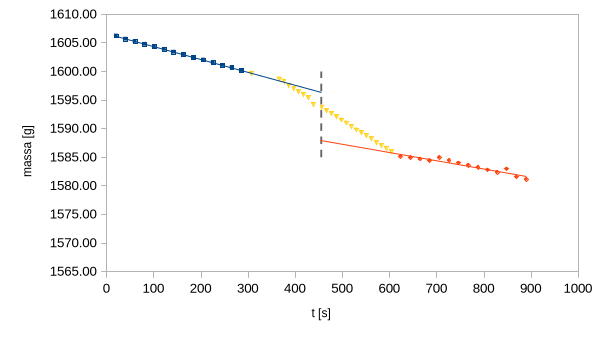
\includegraphics[width=0.85\textwidth]{../Grafici/Graficolatente_1.png}
    
    \caption{\textbf{Andamento della massa in funzione del tempo ed estrapolazione dei background.} 
    I punti sperimentali sono suddivisi cronologicamente nelle tre regioni dell'analisi: 
    i quadrati blu descrivono la Fase I (background termico iniziale a circuito aperto), 
    i triangoli gialli la Fase II (evaporazione indotta per effetto Joule a circuito chiuso) 
    e i rombi arancioni la Fase III (background termico finale a circuito aperto). 
    Le linee continue rappresentano le rette di fit lineare estrapolate rispettivamente in avanti (linea blu) 
    e all'indietro (linea rossa) fino all'istante mediano $t_m = 454.87$ s, evidenziato dalla linea verticale tratteggiata. 
    La discontinuità verticale tra le due rette in corrispondenza di $t_m$ quantifica la massa netta evaporata per solo effetto della potenza elettrica ($\Delta m = 8.464$ g).}
    
    \label{fig:grafico_estrapolazione}
\end{figure}
\subsection{Propagazione dell'Incertezza sulla Massa}
L'incertezza sulla massa estrapolata al tempo $t_m$ per ciascuna fase risente degli errori accoppiati dell'intercetta ($\Delta A$) e della pendenza ($\Delta B$) ricavati dal fit. Nel sistema di riferimento temporale adottato per l'analisi, si ottengono i seguenti contributi:
\begin{align}
\Delta(\Delta m|_{\text{Fase I}}) &= \Delta A_1 + t_m \cdot \Delta B_1 = 0.014506 + 454.865 \cdot (8.6300 \times 10^{-5}) \approx 0.054\text{ g} \\
\Delta(\Delta m|_{\text{Fase III}}) &= \Delta A_3 \approx 0.411\text{ g}
\end{align}
Essendo la Fase III interpolata rispetto alla variabile temporale traslata, l'incertezza all'istante mediano coincide direttamente con l'errore dell'intercetta $\Delta A_3$ calcolato dal software, escludendo l'allargamento fittizio a ventaglio causato dal fattore di proiezione lineare.

L'errore assoluto complessivo sulla massa netta $\Delta(\Delta m)$ si ricava dalla somma diretta dei singoli contributi delle due regioni indipendenti:
\begin{equation}
\Delta(\Delta m) = \Delta(\Delta m|_{\text{Fase I}}) + \Delta(\Delta m|_{\text{Fase III}}) = 0.054\text{ g} + 0.411\text{ g} = 0.465\text{ g}
\end{equation}

\subsection{Calcolo Finale del Calore Latente $\lambda_f$}
Utilizzando i parametri elettrici impostati sul generatore ($V = 8.3\text{ V}$, $I = 0.81\text{ A}$) e la durata effettiva della Fase II ($\Delta t = 296.33\text{ s}$), il valore centrale del calore latente di evaporazione dell'azoto liquido risulta:
\begin{equation}
\lambda_f = \frac{V \cdot I \cdot \Delta t}{\Delta m} = \frac{8.3\text{ V} \cdot 0.81\text{ A} \cdot 296.33\text{ s}}{8.464\text{ g}} \approx 235.39\text{ J/g}
\end{equation}

Assumendo come incertezze strumentali della postazione di misura i valori $\Delta V = 0.1\text{ V}$, $\Delta I = 0.01\text{ A}$ e per il cronometro digitale la sensibilità di $\Delta(\Delta t) = 0.01\text{ s}$, si procede alla propagazione finale dell'errore assoluto $\Delta \lambda_f$:
\begin{equation}
\Delta \lambda_f = \lambda_f \left( \frac{\Delta V}{V} + \frac{\Delta I}{I} + \frac{\Delta(\Delta m)}{\Delta m} + \frac{\Delta(\Delta t)}{\Delta t} \right)
\end{equation}
\begin{equation}
\Delta \lambda_f = 235.39 \cdot \left( \frac{0.1}{8.3} + \frac{0.01}{0.81} + \frac{0.465}{8.464} + \frac{0.01}{296.33} \right) \approx 18.67\text{ J/g}
\end{equation}

Arrotondando il risultato in conformità con le cifre significative dell'incertezza calcolata, la misura finale viene espressa come:
\begin{equation}
\lambda_f = (235 \pm 19)\text{ J/g}
\end{equation}
Il valore di riferimento della letteratura scientifica ($\lambda_{\text{lit}} \approx 199\text{ J/g}$) è pienamente compatibile con l'intervallo di confidenza della misura effettuata, ricadendo all'interno della barra d'errore sperimentale.
\subsection{Calore specifico medio del piombo}






\section{Analisi dati}

\section{Conclusioni}

\end{document}